\documentclass[10pt]{article}
\usepackage[margin=0.8in]{geometry}
\usepackage{booktabs}
\usepackage{graphicx}
\usepackage{parskip}
\usepackage{enumitem}
\usepackage{xcolor}
\usepackage{amsmath}
\usepackage{tikz}
\usetikzlibrary{arrows.meta,positioning}
\usepackage{titlesec}
\usepackage[colorlinks=true,linkcolor=black,urlcolor=blue]{hyperref}
\titleformat{\section}{\normalfont\large\bfseries}{\thesection.}{0.5em}{}
\titleformat{\subsection}{\normalfont\normalsize\bfseries}{\thesubsection.}{0.5em}{}
\setlist[itemize]{leftmargin=1.4em,itemsep=0.15em,topsep=0.25em}
\newcommand{\pass}{\textcolor{green!50!black}{\textbf{PASSED}}}
\newcommand{\fail}{\textcolor{red!70!black}{\textbf{FAILED}}}
\newcommand{\open}{\textcolor{orange!80!black}{\textbf{IN PROGRESS}}}
\tikzset{blk/.style={draw,rounded corners=2pt,minimum width=24mm,minimum height=7mm,font=\scriptsize,align=center},
         ar/.style={-{Stealth[length=1.6mm]}},
         lbl/.style={font=\scriptsize\itshape,align=center}}

\title{\textbf{Dynamics-Modeling Study: Progress Report}\\[2pt]
\large Does predicting object motion make robot policies robust to changed physics?}
\author{}
\date{2026-08-18 \quad (build sessions: 2026-08-16 to 2026-08-18)}

\begin{document}
\maketitle
\vspace{-2.5em}

\section{The experiment in one paragraph}
Train two robot policies that are \emph{identical} except one must also predict how
the object will move (a small ``prediction head'' bolted on during training, deleted
afterwards). Test both under physics they never saw (heavier, slipperier objects).
If the prediction-trained one degrades more slowly, run controlled follow-ups to find
out \emph{why}. Every claim is protected by pre-registered rules and go/no-go gates.

\subsection*{Glossary}
\begin{itemize}
\item \textbf{c} --- the hidden physics of an episode (mass, friction, off-center
weight). The robot feels c but is never told it.
\item \textbf{Teacher} --- a reinforcement-learning agent trained \emph{with} c
visible. It generates expert demonstrations; student policies imitate them blind.
\item \textbf{$\delta$ grid} --- 210 physics settings outside the training range,
used to measure how fast a policy breaks as physics drift.
\item \textbf{Gate} --- a pre-planned go/no-go check. Skipping one silently
invalidates everything after it. Gates failing early and loudly is the design working.
\end{itemize}

\section{Setup and hidden physics}
Simulator: ManiSkill~3 on the PhysX engine; robot: Franka Panda (7-DoF arm +
gripper); thousands of scene copies simulated in parallel per GPU.
Machine: 8$\times$ NVIDIA A100 80\,GB, 96 CPU cores, 1.7\,TB RAM.

\begin{center}
\begin{tabular}{@{}lllll@{}}
\toprule
\textbf{Hidden parameter} & \textbf{Training range} & \textbf{$\delta$-grid values (extended)} \\
\midrule
Mass multiplier & 0.7--1.4 (log-uniform) & 0.3, 0.5, 1.0, 1.6, 2.2, 3.0, 4.5 \\
Surface friction & 0.3--0.7 (log-uniform) & 0.1, 0.2, 0.5, 0.9, 1.2, 1.8 \\
COM offset (frac.\ of half-width) & 0--0.15 (uniform) & 0, 0.10, 0.25, 0.40, 0.60 \\
Granular extras (T1/T2) & 20--30 balls; ball friction 0.2--0.8 & --- (later tier) \\
\bottomrule
\end{tabular}
\end{center}
Grid $=7\times6\times5=210$ points, each tagged interpolation / extrapolation /
composition by how many components leave the training range (2 / 25 / 183 points).
Physics are baked in at scene construction; every episode carries fresh c.

\section{Phase 1: Environments \hfill complete}
\begin{figure}[h]
\centering
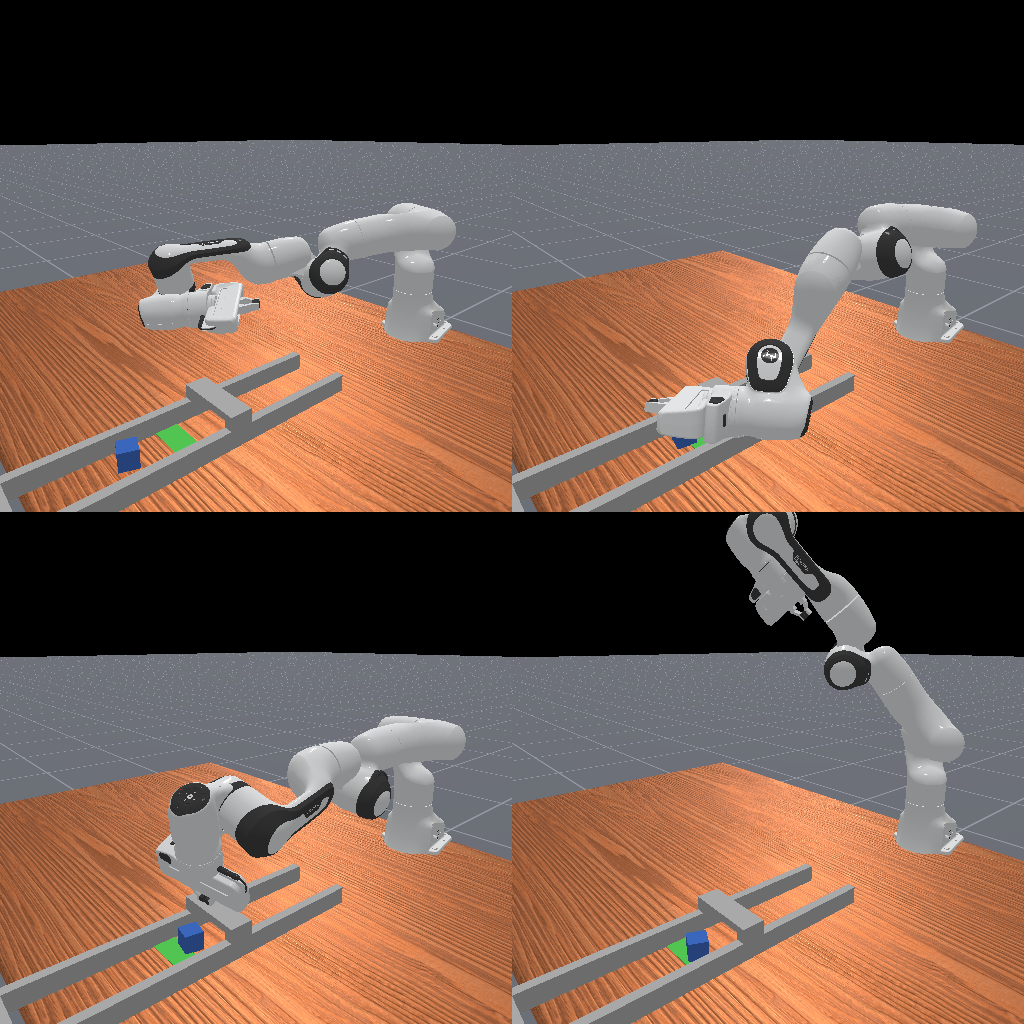
\includegraphics[width=0.48\textwidth]{figs/t3_tunnel.png}\hfill
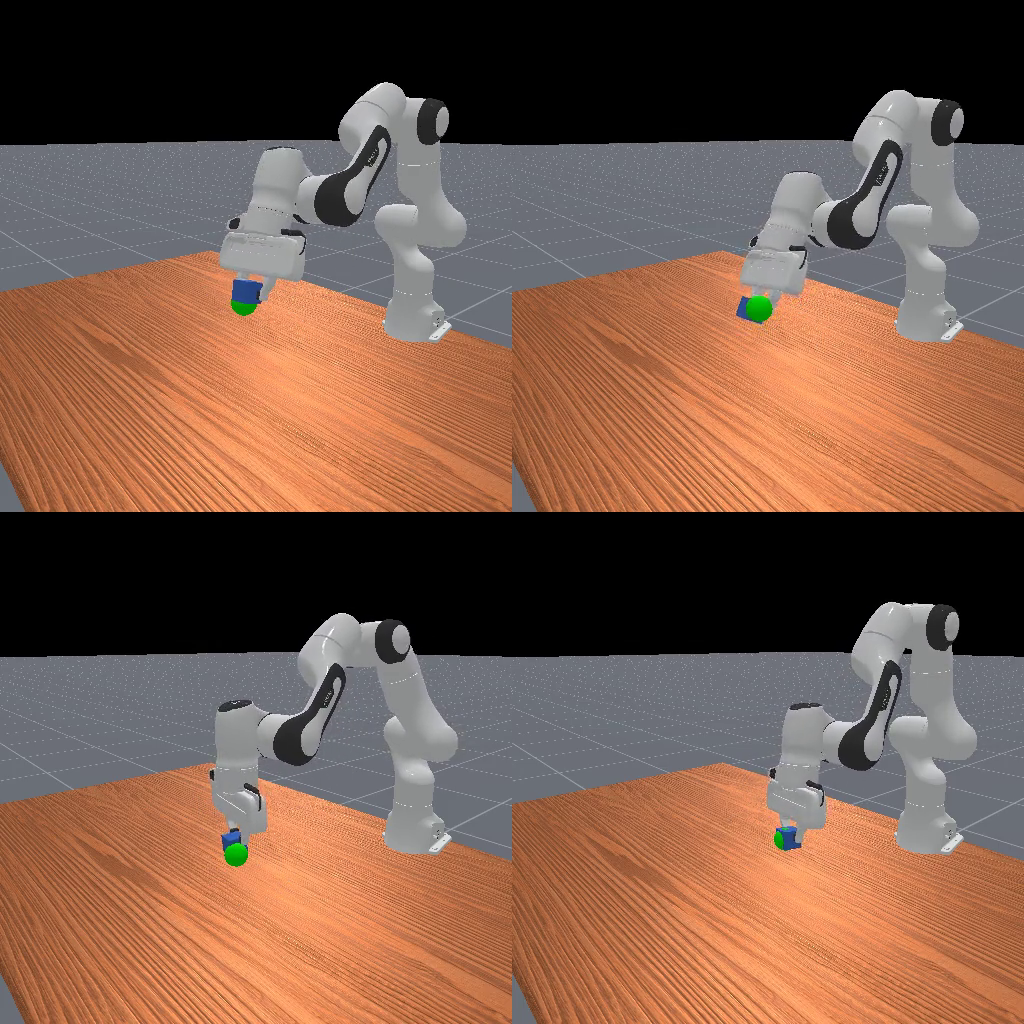
\includegraphics[width=0.48\textwidth]{figs/t4_pickplace.png}
\caption{\textbf{Left, T3 slide-to-slot (primary, with tunnel):} four physics
variants, same controller --- the block stops short, lands in the green slot, or
overshoots depending on hidden mass/friction; the grey crossbar is the tunnel the
hand cannot enter. \textbf{Right, T4 pick-and-place (control):} the trained teacher
holds the cube at the goal in all four variants --- once grasped, physics stop
mattering, by design.}
\end{figure}
\begin{figure}[h]
\centering
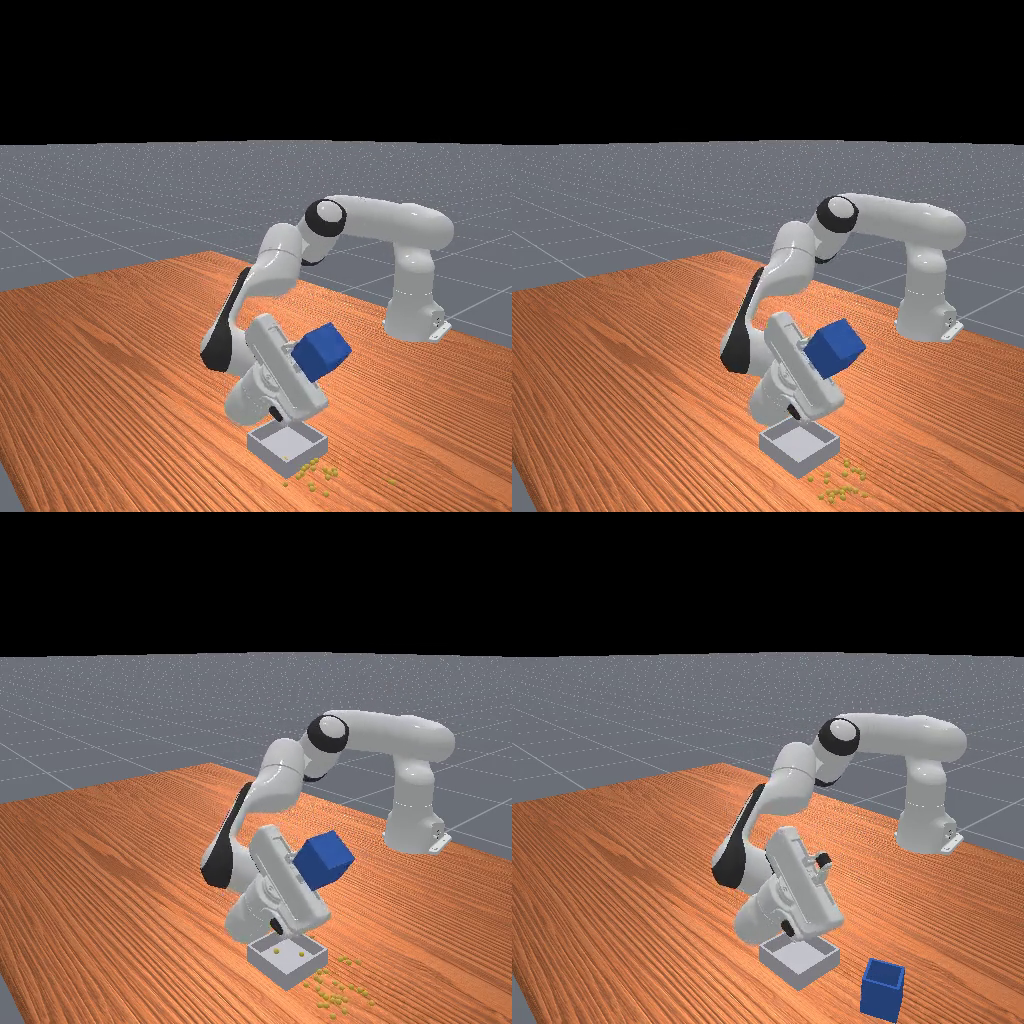
\includegraphics[width=0.48\textwidth]{figs/t1_pour.png}\hfill
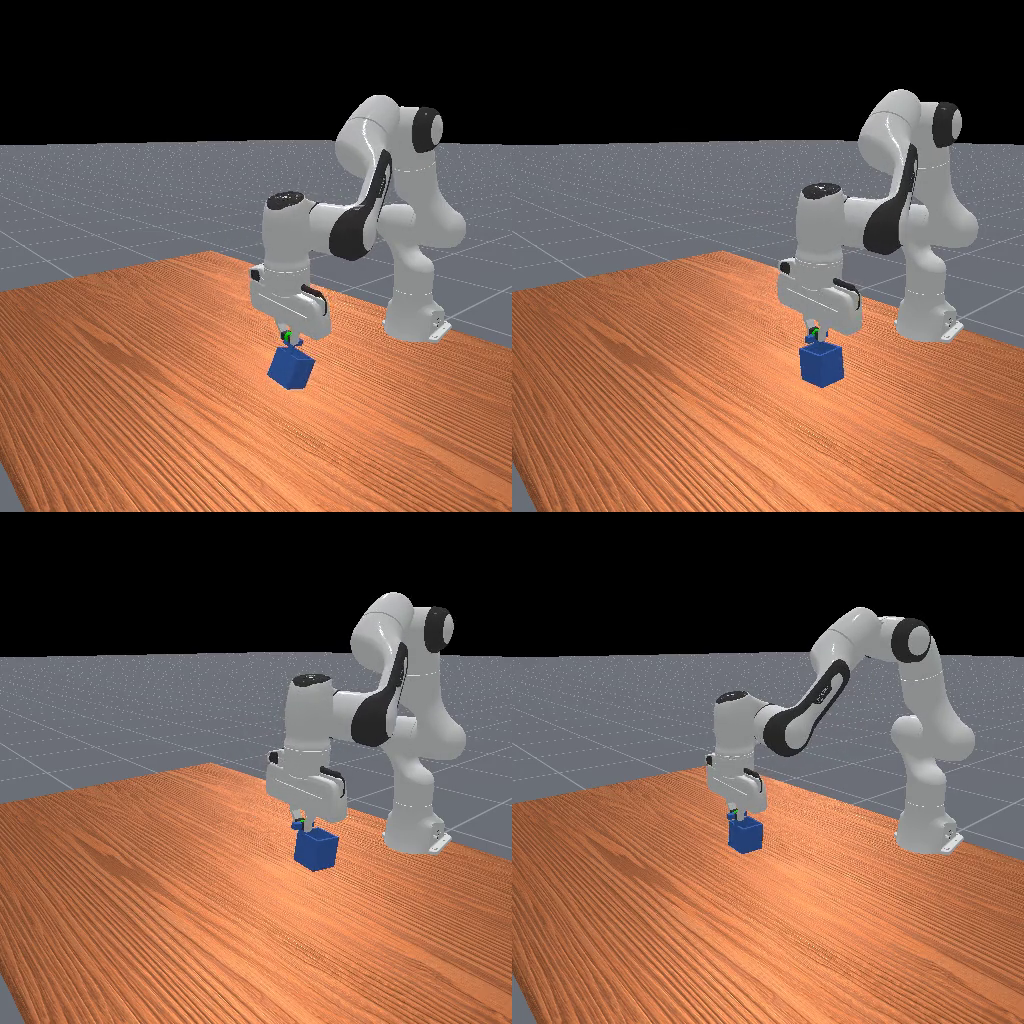
\includegraphics[width=0.48\textwidth]{figs/t2_carry.png}
\caption{\textbf{Left, T1 pouring:} tilt the held cup so its 20--30 balls fall into
the basin --- outflow lags the tilt. One tile shows the grip slipping: a real failure
mode. \textbf{Right, T2 carrying:} the ball-filled mug hangs from the gripper by its
handle; the robot's own acceleration excites the sloshing it must survive. (Harder
tier; environments built and smoke-tested, taken up after T3 reports.)}
\end{figure}

\begin{tabular}{@{}p{7.2cm}p{7.6cm}@{}}
\toprule
\textbf{Check} & \textbf{Result} \\
\midrule
Stock PPO trains end-to-end & \pass{} --- PushCube 100\% eval success \\
Randomization reaches the physics (identical actions, different c) &
\pass{} --- mass alone moves endpoint 8.8\,cm; friction 4.4\,cm; extremes 16\,cm;
COM offset flips rotation. Post-tunnel: 17\,cm spread \\
Teacher obs wider than student obs by exactly c & \pass{} --- +4 dims rigid, +7 granular \\
Granular plumbing (ball counts, retention, held mug) & \pass{} --- mug held 4/4, contents retained \\
\bottomrule
\end{tabular}

\section{Architecture choices (and why)}
\begin{center}
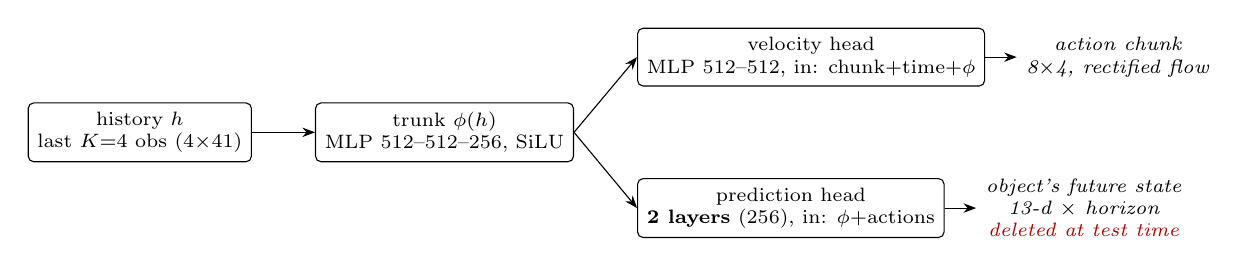
\begin{tikzpicture}[node distance=4mm and 8mm]
\node[blk] (h) {history $h$\\last $K{=}4$ obs (4$\times$41)};
\node[blk,right=of h] (t) {trunk $\phi(h)$\\MLP 512--512--256, SiLU};
\node[blk,above right=2mm and 8mm of t] (v) {velocity head\\MLP 512--512, in: chunk+time+$\phi$};
\node[blk,below right=2mm and 8mm of t] (p) {prediction head\\\textbf{2 layers} (256), in: $\phi$+actions};
\node[lbl,right=4mm of v] (a) {action chunk\\8$\times$4, rectified flow};
\node[lbl,right=4mm of p] (o) {object's future state\\13-d $\times$ horizon\\\textcolor{red!70!black}{deleted at test time}};
\draw[ar] (h)--(t);
\draw[ar] (t.east) -- (v.west);
\draw[ar] (t.east) -- (p.west);
\draw[ar] (v)--(a); \draw[ar] (p)--(o);
\end{tikzpicture}
\end{center}

\textbf{Student policy} ($\sim$1.0M parameters, trained from scratch --- pretrained
weights would break the identical-data constraint):
\begin{itemize}
\item \textbf{Flow matching} (Diffusion-Policy style, rectified-flow objective):
the velocity head learns
$\;\mathcal{L}=\lVert v_\theta(a^\tau,\tau,\phi(h))-(a_1-a_0)\rVert^2$;
at test time 10 Euler steps turn noise into an 8-action chunk, of which the first
4 are executed before re-planning.
\item \textbf{Arm B adds only} $\lambda\lVert g_\theta(\phi(h),a)-x^{\text{obj}}_{t+1..t+H}\rVert^2$.
The head is deliberately \emph{weak} (2 layers): it can only succeed if the physics
information is already in $\phi$ --- a deep head could solve prediction internally
and teach the trunk nothing. It predicts the \emph{object's} state (13-d pose+velocity),
never the robot's joints (those are trivially predictable). Three target types:
one-step, multi-step ($H{=}8$), latent (stop-gradient). Verified: A and B are
byte-identical at deployment.
\item \textbf{Controls}: B-shuffled (targets randomly permuted --- one line) and
arm C (forecast concatenated to $\phi$ at inference, as published hybrids do).
\end{itemize}

\textbf{Teacher} (PPO, stock script, only the observation changed): actor--critic,
each a 3$\times$256 tanh MLP; input $=$ student obs (41) $+$ c (4).

\begin{center}
\begin{tabular}{@{}llll@{}}
\toprule
\multicolumn{2}{@{}l}{\textbf{Student training}} & \multicolumn{2}{l@{}}{\textbf{Teacher training (PPO)}} \\
\midrule
optimizer & AdamW, lr $3{\cdot}10^{-4}$, cosine & parallel envs & 2048 \\
batch / steps & 256 / 60k & discount $\gamma$ / GAE $\lambda$ & 0.97 / 0.95 \\
checkpoints & 15, log-spaced (for emergence curves) & episode end & \emph{not} on success (anti-hover) \\
obs normalization & per-dataset mean/std & steps per attempt & 50--75M ($\sim$1\,h) \\
\bottomrule
\end{tabular}
\end{center}

\section{Data: what exists and how much}
Each demonstration episode stores per-step observations (41-d, c provably absent),
actions, rewards, success flags, and full simulator state (replayable later into
camera images --- that is how the vision variant is made without regenerating).
c goes to a separate metadata file, one row per episode.

\begin{center}
\begin{tabular}{@{}lrrrl@{}}
\toprule
\textbf{Dataset} & \textbf{Episodes} & \textbf{Transitions} & \textbf{Size} & \textbf{Status} \\
\midrule
T4 teacher demos & 10{,}000 & 0.8M & 415\,MB & complete, verified (99.7\% success) \\
T3 teacher demos $10^3$/$10^4$ & 11{,}000 & 2.2M & 1.07\,GB & \emph{invalidated by tunnel; regenerate} \\
T3 teacher demos $10^5$ & 100{,}000 & 20M & $\sim$10\,GB & regenerate after new teacher \\
c-blind set $10^3$/$10^4$ & 11{,}000 & 2.2M & 1.03\,GB & \emph{invalidated; expert rebuilt, ready} \\
Scripted warm-start set & 4{,}000 & 0.8M & 375\,MB & complete (46\% success, tunnel era) \\
Vision variant ($10^4$, 128$\times$128 RGB) & 10{,}000 & 2M & $\sim$1\,TB & pipeline verified; generate at vision stage \\
Evaluation manifest & 210{,}000 & --- & --- & fixed episode seeds, all arms identical \\
\midrule
\multicolumn{2}{@{}l}{Teacher RL experience (not stored)} & $\sim$230M & --- & across 6 T3 attempts + T4 \\
\bottomrule
\end{tabular}
\end{center}

\section{Teachers: six attempts, every failure diagnosed}
T4 was clean first try: 99.6\% success, spread 0.03 across c (\pass{}); its
dataset is done. T3's history \emph{is} the robustness story:

\begin{tabular}{@{}p{0.7cm}p{6.7cm}p{7.2cm}@{}}
\toprule
\textbf{v} & \textbf{Problem found} & \textbf{Fix} \\
\midrule
v1 & Default RL discount too short-sighted for a 200-step task & $\gamma$ 0.8$\to$0.97 \\
v2 & \textbf{Hovering bug}: ending episodes at success cut the reward stream;
lingering at the edge of success out-paid finishing (eval $0.0$ vs train $0.94$) &
Episodes continue past success; the success state keeps paying, so finishing dominates \\
v2b & Last checkpoint worse than best (0.69 vs 0.91, late-RL decay); flatness looked
failed but the cell spread matched pure binomial noise & Certify best checkpoint by
eval; flatness judged on per-axis marginals ($\le$3.5 pts on every axis)
$\Rightarrow$ \pass{} at 92.4\% \\
\multicolumn{3}{@{}l@{}}{\emph{--- tunnel redesign (Section 7) invalidated the above; new task, new teacher ---}} \\
v3 & 4\%: a precise 24\,cm blind flick is undiscoverable by exploration noise & Tunnel moved to sit just before the slot \\
v4 & Launch-speed reward bonus alone did not help (still 4\%) & superseded by v5 geometry \\
v5 & Plateau at $\sim$18\%: flick technique still rare under exploration & kept running as fallback \\
v6 & --- & \textbf{Warm start}: behavior-clone the scripted expert's successful
flicks into the PPO network, then fine-tune with c visible. \open{}: 27\% at 6M
steps --- already past v5's 41M-step plateau \\
\bottomrule
\end{tabular}

\begin{figure}[h]
\centering
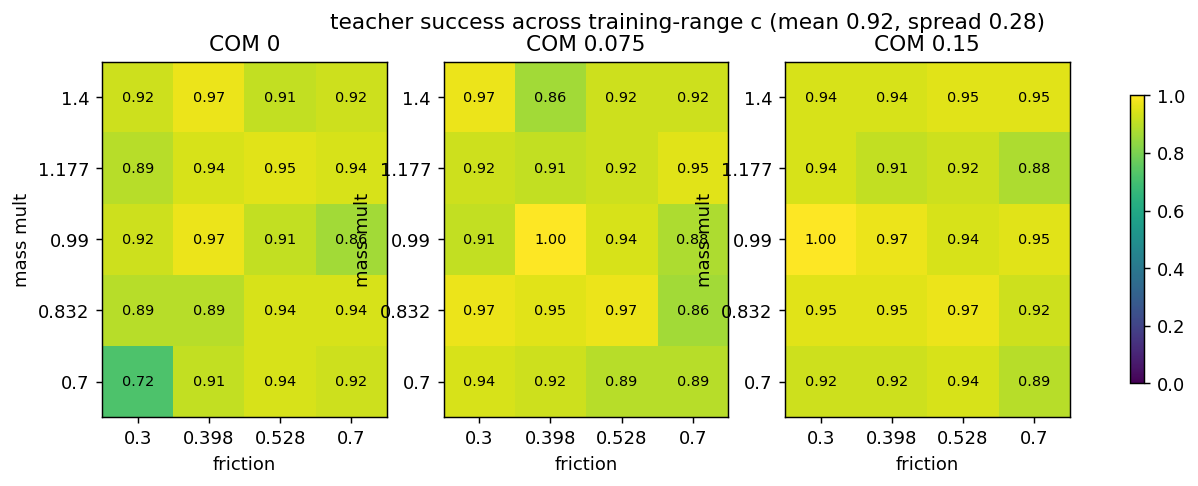
\includegraphics[width=0.9\textwidth]{figs/flatness.png}
\caption{The flatness gate in action (pre-tunnel teacher shown): success rate over
the full training range of c --- mass $\times$ friction panels at three COM levels,
64 episodes per cell. The surface is flat within noise; per-axis averages differ by
$\le$3.5 points. A teacher failing this check would poison part of physics-space
with weak demonstrations.}
\end{figure}

\section{The central finding: the escorting exploit and the tunnel}
A required gate: before the experiment runs, the plain policy must \emph{visibly
fail} under extreme physics, else there is no gap to explain. It refused to fail
(0.92 in-range $\to$ 0.80 at extremes; the continuous distance measure plateaued
too). Instrumentation found the cause: the gripper stayed within 6\,cm of the
object for $\sim$80\% of the final approach --- \textbf{escorting}. Continuous
contact $=$ continuous correction $=$ physics never matter.

\textbf{Fix: the tunnel} (visible in Fig.~1) --- a roof over the channel directly
before the slot; the object slides under, the hand cannot. The final stretch is now
a committed free slide whose stopping point c decides, while both recovery
directions survive. Verified: identical launches now spread outcomes across
\textbf{17\,cm}. Follow-on mechanics, found cheaply with the scripted expert:
launches need a \emph{run-up} (a strike from standstill enters at half speed and
dies under the roof at every strength); with a 13\,cm charge, one \emph{fixed}
flick reaches 43--46\% success. That controller became both the rebuilt c-blind
demonstrator and v6's warm start.

\section{Measurement tools, validated the hard way}
Probes (small readouts measuring how much physics knowledge a policy's internals
hold) and ablations (deleting it) had to pass a gate on the calibration tier,
where ground truth is known. Five failures, each a real trap caught on a toy:
(1)~no excitation --- the expert settles the system and physics vanish from data;
(2)~shortcut learning --- imitation via a ratio trick, no physics represented;
(3)~an under-identified system --- the optimal gain barely varied with physics
(variance 0.05), nothing to decode; (4)~query-entangled features --- probe
directions did not transfer; (5)~\textbf{redundant encodings defeat linear
erasure} --- after deleting 16 directions the quantity stayed readable
(R$^2$ 0.60--0.82) and the deletion hurt no more than deleting random directions,
while the decoy control stayed exactly null. Final state: \pass{}, with a
pre-registered consequence: \textbf{ablation results count as evidence only when
positive}.

\section{Robustness practices in force}
\begin{itemize}
\item Arms differ by exactly one loss term; same data, architecture, parameter
count, optimizer, seeds. Students trained from scratch.
\item Pre-registration (\texttt{configs/preregistration.json}): falsification rule
(overlapping 95\% CIs on A-vs-B degradation slopes over $\ge$10 seeds $=$ no
effect, and that is the reported result), $\lambda$-sweep spec (20 values
$\times$ 5 seeds), substitution budgets (exactly 12 configs per rival mechanism,
closing criterion $|s_{\text{sub}}-s_{\text{treat}}| < 0.25\,|s_{\text{base}}-s_{\text{treat}}|$),
ablation interpretation rule --- all frozen before any arm runs; amendments dated.
\item Fixed evaluation seeds; interpolation / extrapolation / composition reported
separately, never averaged; binary success \emph{and} continuous distance logged
(success saturates and can hide differences).
\item Measured limitation: GPU physics repeats only to $\sim$4\,cm on violent
launches --- absorbed by many episodes per grid point.
\item Every gate output archived in \texttt{reports/}; every failure documented
(this report, \texttt{PROGRESS.md}); task/protocol changes only before arm launch.
\end{itemize}

\section{Status, compute, and what remains}
Measured throughput: simulation $\sim$13k env-steps/s per GPU (PPO);
one student run $\sim$20\,min; one full $\delta$-grid evaluation (210 points
$\times$ 20 episodes) $\sim$10\,min. Launcher packs 3 runs per 80\,GB GPU
$\times$ 8 GPUs $=$ 24 concurrent.

\begin{enumerate}[leftmargin=1.6em,itemsep=0.1em]
\item \open{} Teacher v6 (warm-started) vs v5 (fallback); first to pass the
flatness gate becomes the data factory.
\item Regenerate T3 datasets ($10^3$/$10^4$/$10^5$) and the c-blind set ($\sim$2\,h).
\item Fresh arm A $\to$ re-run the decisive gate: it must now \emph{fail} at
extreme physics. (If not: extend the grid or shorten history, per plan.)
\item The 180-run matrix (6 arm variants $\times$ 10 seeds $\times$ 3 data scales,
$\sim$3\,h) $\to$ evaluations ($\sim$6\,h) $\to$ slope comparison $=$ headline answer.
\item $\lambda$ sweep (100 runs); substitution arms (240 runs) only if the effect
exists; probes + emergence curves from the log-spaced checkpoints.
\item Later tier: T1/T2 teachers, vision-based arms ($\sim$1\,TB data step).
\end{enumerate}

\textbf{Where things live}: code \texttt{dynmod/} (README maps every plan item to a
file); gates \texttt{reports/}; rules \texttt{configs/}; running log
\texttt{PROGRESS.md}; figures \texttt{figs/}; big files
\texttt{/mnt/scratch/dynamics/} (wiped on shutdown --- backed up to
\texttt{scratch\_backup/}). Weights \& Biases mirroring is wired into every
training run (\texttt{--track}); needs a one-time \texttt{wandb login}.

\end{document}
